\documentclass[a4paper]{article}

%--------------------------------------------------------------------------
\usepackage[a4paper, total={6in, 9in}]{geometry}
\usepackage{amsmath}
\usepackage{booktabs}
\usepackage{caption}
\usepackage{enumitem}
\usepackage{graphicx}
\usepackage{float}
\usepackage{inconsolata}
\usepackage{listings}
\usepackage{pstricks-add}
\usepackage{siunitx}
\usepackage[most]{tcolorbox}
\usepackage{tikz}

\usetikzlibrary{shapes.geometric}

%--------------------------------------------------------------------------
\graphicspath{{./fig/}}

%--------------------------------------------------------------------------
\newtcblisting[auto counter]{sexylisting}[2][]{sharp corners, 
    fonttitle=\bfseries, colframe=gray, listing only, 
    listing options={basicstyle=\ttfamily,language=Python}, 
    title=Listing \thetcbcounter: #2, #1}

%--------------------------------------------------------------------------
\begin{document}
\title{Udacity: 3D Perception Report}
\author{Shane Reynolds}
\maketitle
\section{Introduction \& Background}
In order for a robot to perform meaningful actions it requires some capacity to perceive its environment - the devices used to capture data about an environment are called sensors. There are two main categories into which sensors fall into: active, and passive. The principal distinction between these two types of sensors are that passive sensors measure energy which is already present in the environment, whilst active sensors emit some form of energy and measure the reactions of this energy with the environment. Table 1 (over the page) shows some examples of the more common sensors which are used for robotic perception. Generally, robotic perception systems are comprised of both active and passive sensors. In fact, both active and passive sensors are often combined into a single sensor to create a hybrid sensor. An example of a widely used hybrid sensor which features in many households is the Microsoft Kinect, shown in Figure 1.

\begin{figure}[h]
\centering
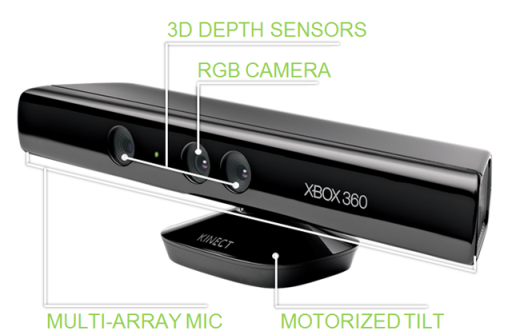
\includegraphics[scale=0.3]{image1}
\caption{The Microsoft Kinect is an example of a hybrid sensor called an RGBD camera. It captures 2D pixel arrays in 3 colour channels, in addition to capturing depth information using structured infra-red light pattern.}
\end{figure}

This project explores the perception of an environment using a hybrid sensor called an RGBD camera. This type of sensor captures a 2D pixel array on red, green, and blue channels using a monocular camera. Further, the sensor captures depth information by measuring the deformation of reflections from structured infra-red (IR) light emitted into the environment. The sensor will be employed using a WillowGarage PR2 robot simulated using ROS, Gazebo, and Rviz. A real world image of the PR2 can be seen in Figure 2, and a close up of the robot's sensing hardware can be seen in Figure 3.

\begin{figure}[H]
\centering
\begin{minipage}[t]{0.45\linewidth}
\centering
\frame{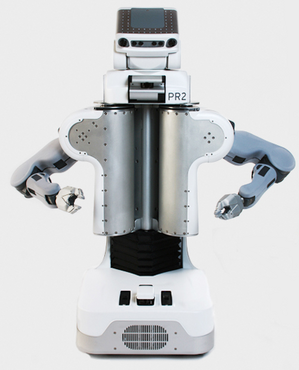
\includegraphics[height=3.3cm]{image2}}
\caption{A picture of the WillowGarage PR2 robot.}
\end{minipage}
\hspace{0.5cm}
\begin{minipage}[t]{0.45\linewidth}
\centering
\frame{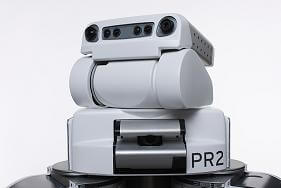
\includegraphics[height=3.3cm]{image3}}
\caption{A close up of the PR2's RGBD camera which captures image and depth data, and is used to create point clouds.}
\end{minipage}
\end{figure}

\begin{table}[h]
\centering
\caption{Examples of passive and active sensors which can be used for robotic perception systems (note that this list is not exhaustive)}
\begin{tabular}{p{2.3cm}p{4.5cm}p{2.3cm}p{4.5cm}}
\toprule
\multicolumn{2}{c}{\textbf{Passive Sensors}} & \multicolumn{2}{c}{\textbf{Active Sensors}}\\
\cmidrule(lr){1-2} \cmidrule(lr){3-4}
\textbf{Name} & \textbf{Description} & \textbf{Name} & \textbf{Description}\\
\midrule
Monocular Camera & A single RGB camera providing information on texture and shape & LIDAR & A 3D laser scanner which determines information about an environment through reading pulsed laser emission reflections\\
& & & \\
Stereo Camera & Consists of 2 monocular cameras providing the same information as the single monocular camera, but with the addition of depth information too & Time of Flight Camera & A 3D ToF camera performs depth measurement by illuminating environment with infra-red and observing the time taken to reflect from surfaces to the camera\\
& & & \\
& & Ultrasonic & Provides depth information by sending out high-frequency sound pulses and measuring time taken for sound to reverberate\\
\bottomrule
\end{tabular}
\end{table}

The captured sensor information is processed into a point cloud using the \verb|pcl| library which is implemented in ROS. Perception of an environment is not simply the capture of point cloud data, rather, it is the implementation of software in order to make sense of the point cloud data. The ultimate goal of this project is for the PR2 to identify objects on a table, pick these objects in a specified order, and stow them into the desired container either on the left or the right of the robot. In order to complete this task, there are two main sub-tasks that the robot's perception architecture must achieve: Segmentation, and Object Recognition. Segmentation is a complex process made up of many subtasks. Briefly, the segmentation implementation for this project is made up of the following sequence of activities:
\begin{enumerate}
\item Statistical filtering;
\item Voxel downsampling;
\item RANSAC plane filtering;
\item Passthrough filtering; and
\item Euclidean clustering (DBSCAN)
\end{enumerate}

These activities are applied to the captured point cloud data, and will be explored in more detail in Section 2.1. Object recognition is a similarly complex activity, which employs the uses of machine learning. There are numerous machine learning schemes that may be implemented in this instance, to varying degrees of effectiveness and computational cost. Irrespective of which machine learning algorithm is used, features which will be important to the developed model will need to be selected, and data captured which is used to train the model. This project employs the use of a supervised learning algorithm called a support vector machine and will be explored in more detail in Section 2.2.

\newpage

%--------------------------------------------------------------------------
\section{Methods \& Implementation}
\subsection{Segmentation}
\subsubsection{Statistical Filtering to Remove Image Noise}
As previously mentioned, the point cloud is obtained using an RGBD camera to capture a 2D image which consists of three feature maps, and a depth representation. The three feature maps represent the individual Red, Green, and Blue (RBG) channels for colour image. Each discrete pixel in the 2D array is also assigned an image depth. There are a total of 4 dimensions for each individual point in the point cloud which is assembled in the ROS environment by the \verb|pcl| library. The captured point cloud is not a perfect representation of the environment, rather, there are elements of noise introduced through dust, humidity, and light sources in the environment. Further, often instrumentation and transmission channels are imperfect which produce noise in the signal. The noisy signal can be seen in Figure 4 - the noise are the stochastic particles throughout the image. To remove the noise, a statistical outlier filter is used. This employs a Gaussian method to remove statistical outlier from the pointcloud. The implementation in the \verb|pcl_callback| function can be seen in Listing 1. A signal which has had noise removed can be seen in Figure 5. The successful implementation of the object recognition relies on clean segmentation of objects in a frame. The presence of noise results in the confusion of the Euclidean clustering method which provides segmentation, so it is important to apply this statistical filter prior to any further processing.

\vspace{1cm}

\begin{figure}[h]\scriptsize
\begin{sexylisting}{Obtain the point cloud and statistically filter to remove noise}
##############################################################################
    # Convert ROS msg to PCL data
##############################################################################
    cloud = ros_to_pcl(pcl_msg)

##############################################################################
    # Statistical Outlier Filtering
##############################################################################
    outlier_filter = cloud.make_statistical_outlier_filter()
    outlier_filter.set_mean_k(2)
    outlier_filter.set_std_dev_mul_thresh(0.5)
    cloud_filtered = outlier_filter.filter()
\end{sexylisting}
\end{figure}

\vspace{1cm}

\begin{figure}[h]
\centering
\begin{minipage}{0.45\linewidth}
\centering
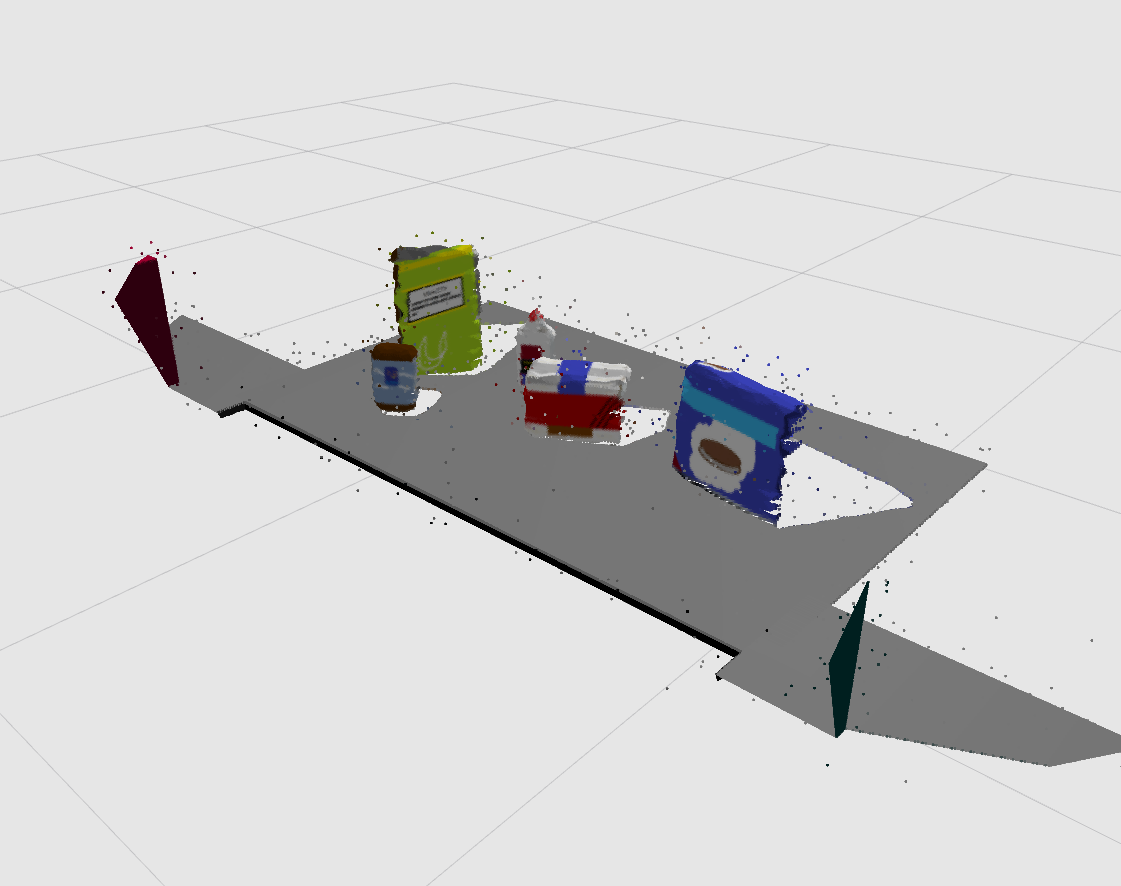
\includegraphics[scale=0.2]{image11}
\caption{Noisey point cloud of table and objects}
\end{minipage}
\hspace{0.5cm}
\begin{minipage}{0.45\linewidth}
\centering
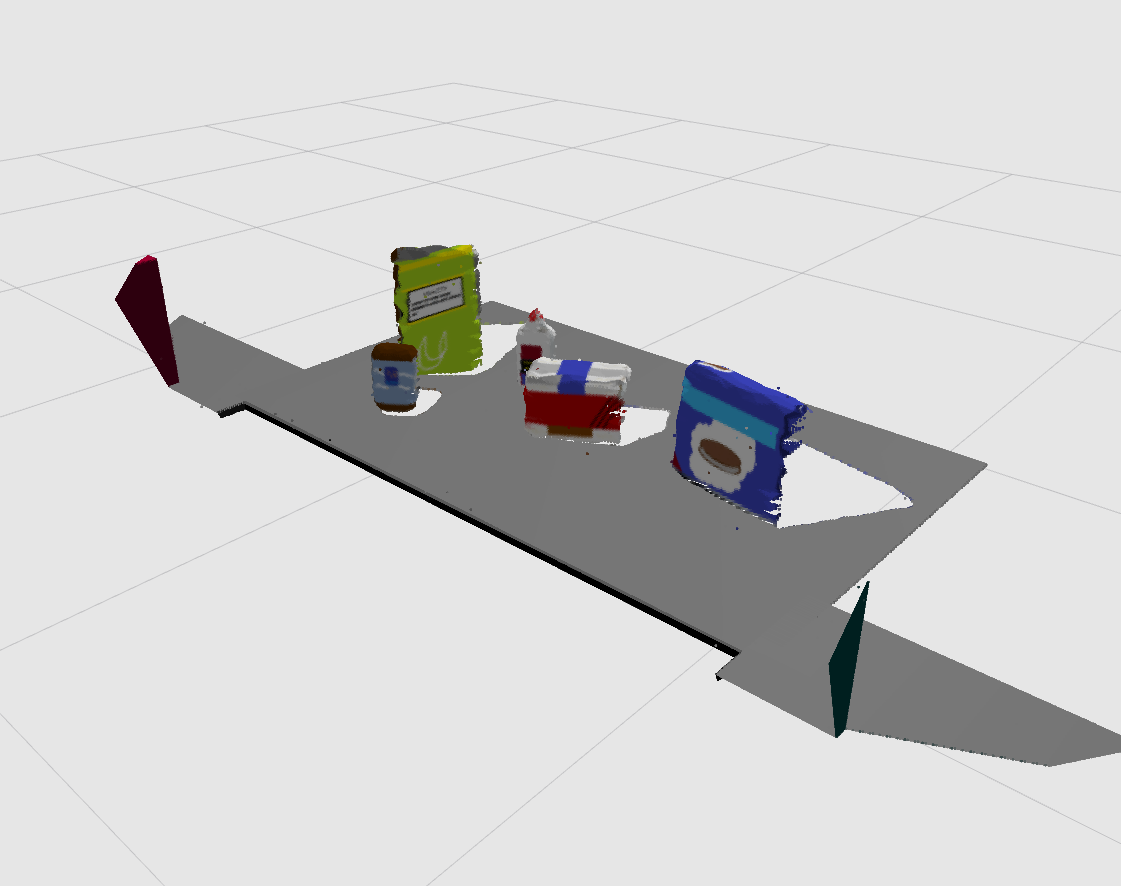
\includegraphics[scale=0.2]{image5}
\caption{The application of the Gaussian filter removes noise from the signal}
\end{minipage}
\end{figure}

\newpage

\subsubsection{Voxel Downsampling}
Point clouds often provide more data than necessary to achieve an accurate representation of the physical environment. The processing of this data, left unchecked, is computationally expensive. Downsampling is the process of removing data points in a systematic fashion, and is a technique that is often employed in the field of image processing. Voxel downsampling is analogous to the 2D process, that is, points in the three dimensional point cloud model are removed in a systematic fashion. Care needs to be taken when adjusting the parameters for the Voxel downsampling - if the downsampling is too aggressive, too much information may be removed compromising the ability to provide effective segmentation. The implementation of the Voxel downsampling can be seen in Listing 2. Figure 6 shows the pointcloud before Voxel downsampling, and Figure 7 shows the pointcloud after downsampling.

\vspace{1cm}

\begin{figure}[h]\scriptsize
\begin{sexylisting}{Obtain the point cloud}
##############################################################################
    # Voxel Grid Downsampling
##############################################################################
    # Create a VoxelGrid filter object for our input point cloud
    vox = cloud_filtered.make_voxel_grid_filter()

    # Choose a voxel (also known as leaf) size
    LEAF_SIZE = 0.01

    # Set the voxel (or leaf) size
    vox.set_leaf_size(LEAF_SIZE, LEAF_SIZE, LEAF_SIZE)

    # Call the filter function to obtain the resultant downsampled point cloud
    cloud_filtered = vox.filter()
\end{sexylisting}
\end{figure}

\vspace{1cm}

\begin{figure}[h]
\centering
\begin{minipage}{0.45\linewidth}
\centering
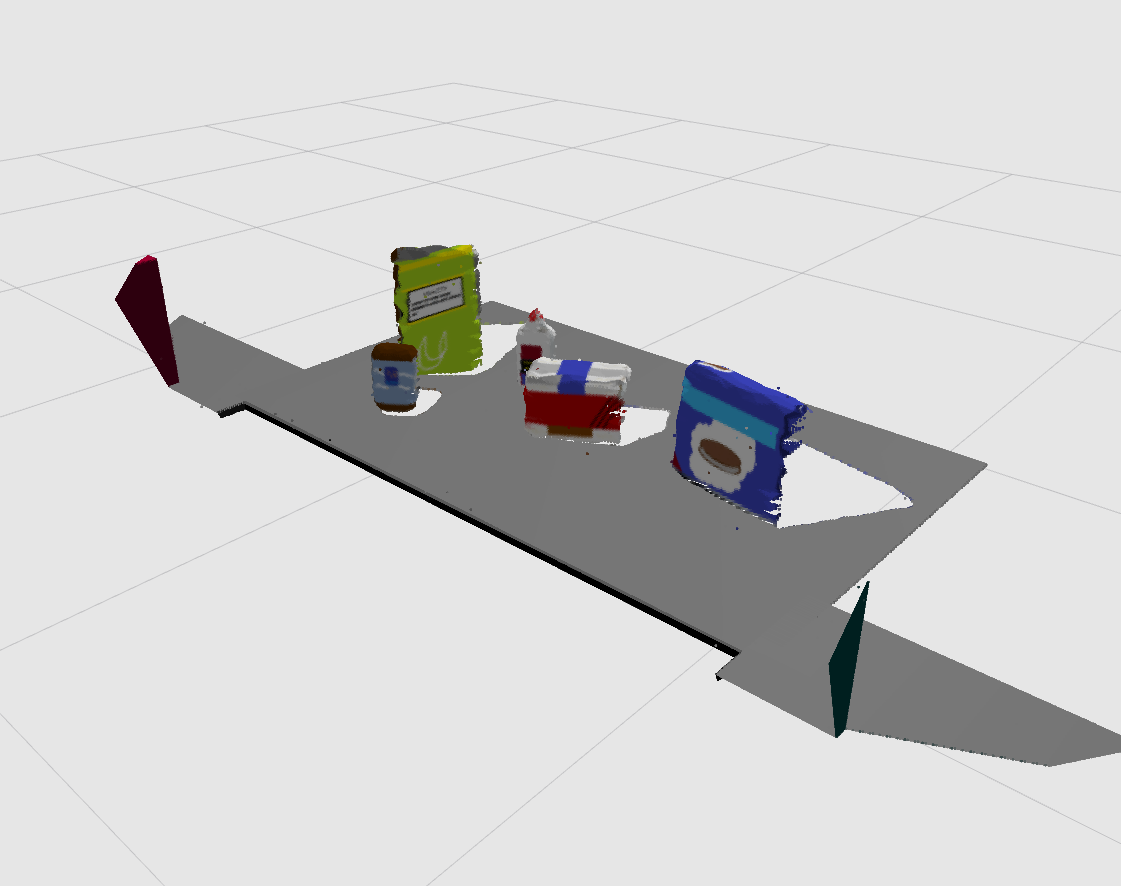
\includegraphics[scale=0.2]{image5}
\caption{include a figure which shows no Voxel Downsampling}
\end{minipage}
\hspace{0.5cm}
\begin{minipage}{0.45\linewidth}
\centering
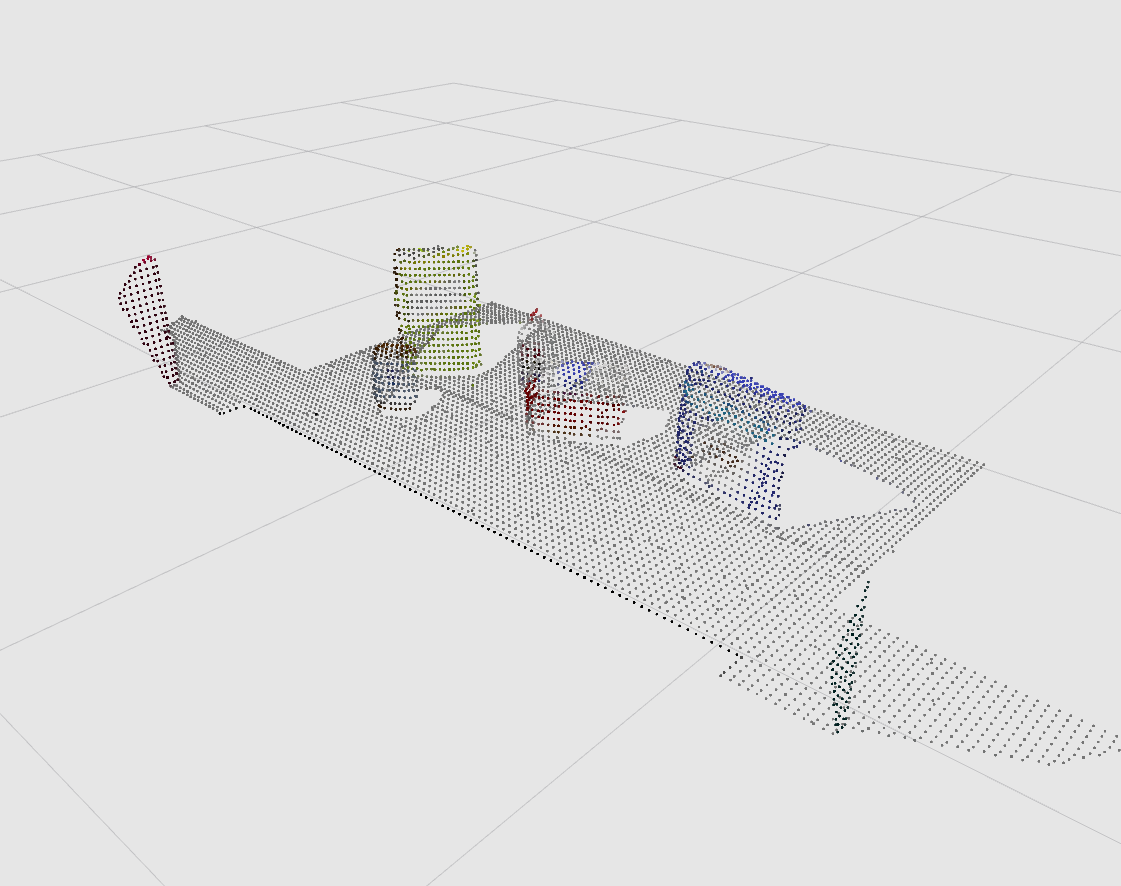
\includegraphics[scale=0.2]{image10}
\caption{include a figure which shows the basics of Voxel Downsampling}
\end{minipage}
\end{figure}

\newpage

\subsubsection{Passthrough Filtering}
A pass through filter is a simply designed to remove points from the point cloud which fall outside a spatially bounded region. This filter is very basic in its implementation, and does not rely on any statistical filters to achieve the results. The implementation can be seen in Listing 4. In this instance, we remove points which don't fall within an area bounded by a rectangular prism. Whilst this filtering is not essential, it helps stops the robot from segmenting points which belong to the boxes which lie to the left and right of the robot's work space. It also removes the robot's arms from the point cloud. Figure 8 shows the unfiltered pointcloud, and Figure 9 shows the pointcloud after the passthrough filter has been applied.

\vspace{1cm}

\begin{figure}[h]\scriptsize
\begin{sexylisting}{Obtain the point cloud}
##############################################################################
    # PassThrough Filter
##############################################################################
    # Create a PassThrough filter object.
    passthrough_z = cloud_filtered.make_passthrough_filter()

    # ZAXIS Assign axis and range to the passthrough filter object.
    filter_axis = 'z'
    passthrough_z.set_filter_field_name(filter_axis)
    axis_min = 0.60
    axis_max = 1.8
    passthrough_z.set_filter_limits(axis_min, axis_max)

    # Use the filter function to obtain the filtered z-axis.
    cloud_filtered = passthrough_z.filter()

    # Create PassThrough filter object
    passthrough_y = cloud_filtered.make_passthrough_filter()

    # YAXIS Assign axis and range to the passthrough filter object
    filter_axis = 'y'
    passthrough_y.set_filter_field_name(filter_axis)
    axis_min = -0.5
    axis_max = 0.5
    passthrough_y.set_filter_limits(axis_min, axis_max)

    # Use the filter function to obtain the filtered y-axis
    cloud_filtered = passthrough_y.filter()
\end{sexylisting}
\end{figure}

\vspace{1cm}

\begin{figure}[h]
\centering
\begin{minipage}{0.45\linewidth}
\centering
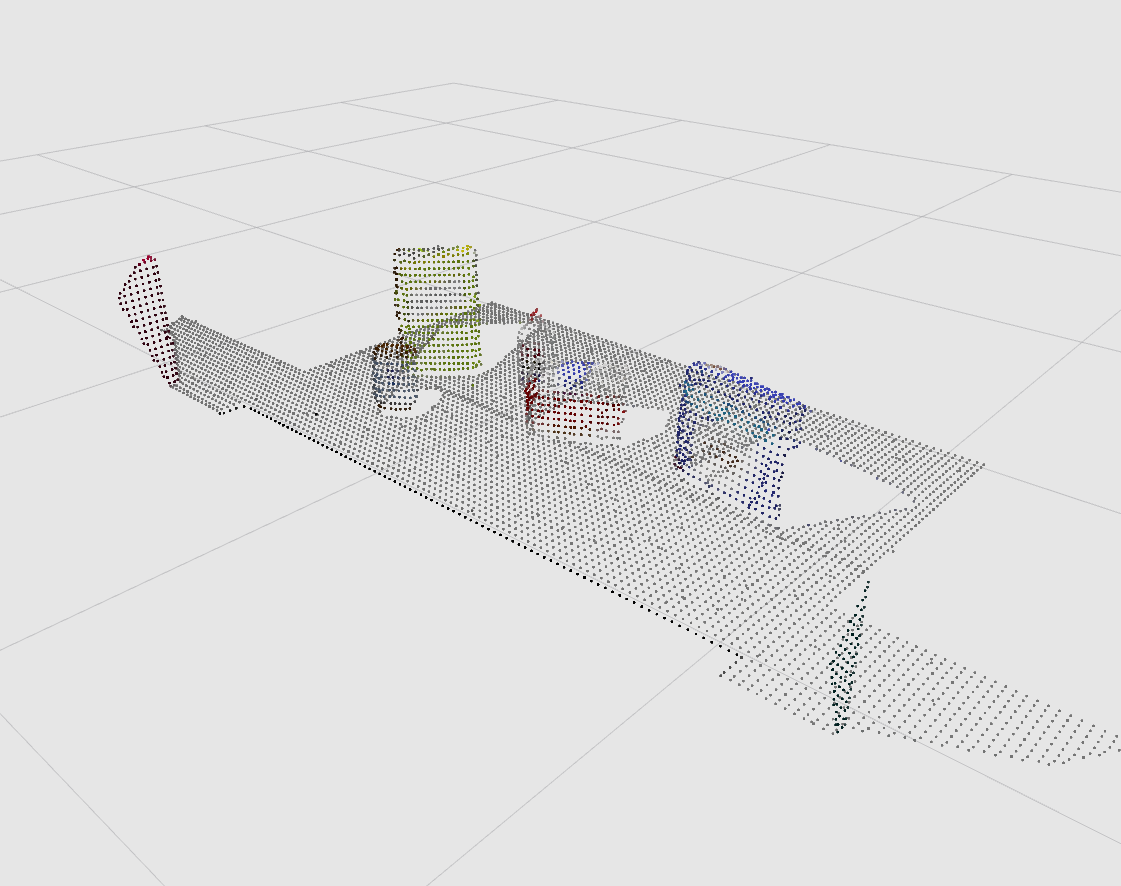
\includegraphics[scale=0.2]{image10}
\caption{Include and image of the unfiltered point cloud}
\end{minipage}
\hspace{0.5cm}
\begin{minipage}{0.45\linewidth}
\centering
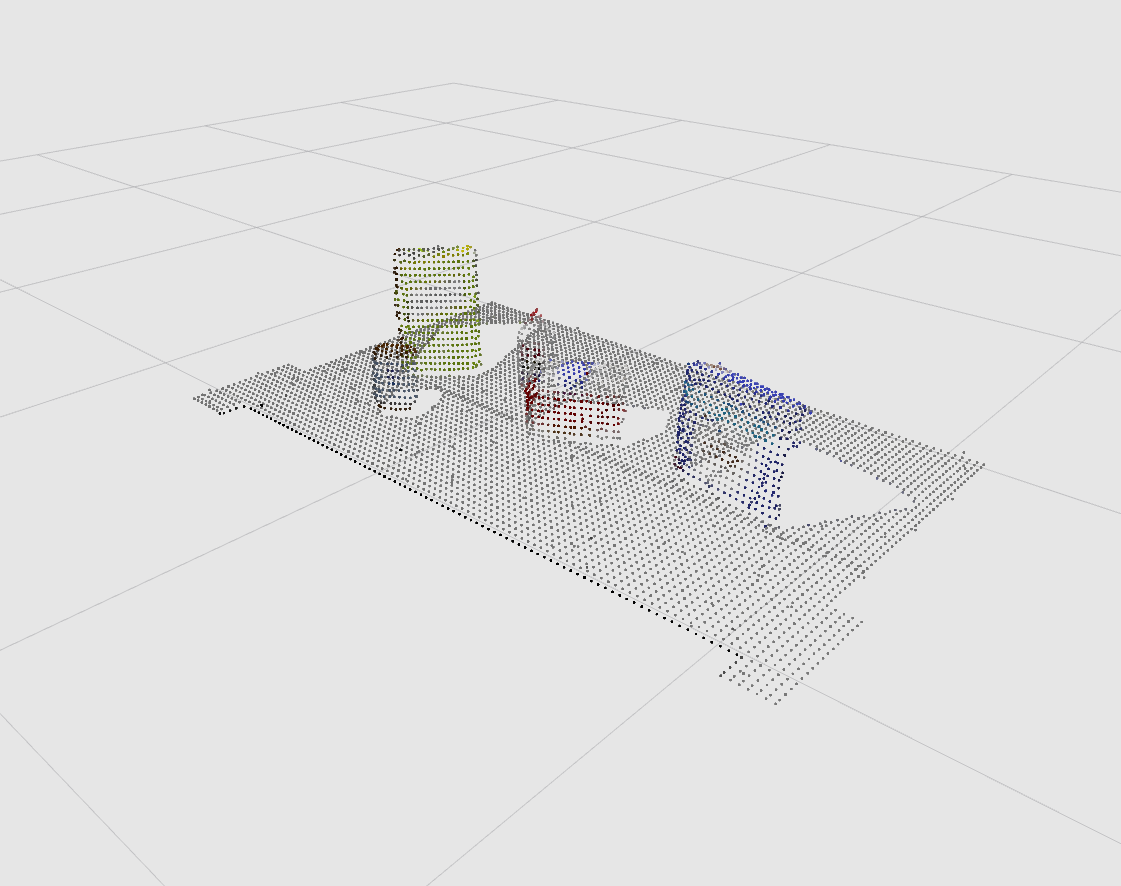
\includegraphics[scale=0.2]{image7}
\caption{Include an image of the filtered point cloud}
\end{minipage}
\end{figure}

\newpage

\subsubsection{RANSAC Plane Segmentation}
Random sample consensus (RANSAC) is an segmentation algorithm which detects statistical outliers which do not fit a geometrical mathematical model. The mathematical model is specified depending on the filtering requirement. In this instance the mathematical model being used is a plane, which closely resembles the table which the objects sit on in the point cloud image. The model outliers, that is those points which don't statistically fit the mathematical representation of a plane, are filtered from the point cloud. Filtered points which fit the model are stored in the variable \verb|could_table|, and those that don't fit the model are stored in the variable \verb|cloud_objects|. This processing helps to isolate the objects in the image, ready for segmentation and object recognition. The implementation can be seen in Listing 4. The filtered could points which fit the model can be seen in Figure 10 - the table has been extracted. The remaining points, the outliers, can be seen in Figure 11. Including the table in the pointcloud image creates a potential opportunity to confuse the Euclidean clustering algorithm since the segmentation is based on spatial proximity. Further benefits include the decreased computation cost for processing the remainder of the point cloud.

\vspace{0.25cm}

\begin{figure}[h]\scriptsize
\begin{sexylisting}{Obtain the point cloud}
##############################################################################
    # RANSAC Plane Segmentation
##############################################################################
    # Create the segmentation object
    seg = cloud_filtered.make_segmenter()

    # Set the model you wish to fit
    seg.set_model_type(pcl.SACMODEL_PLANE)
    seg.set_method_type(pcl.SAC_RANSAC)

    # Max distance for a point to be considered fitting the model
    max_distance = 0.01
    seg.set_distance_threshold(max_distance)

    # Call the segment function to obtain set of inlier indices and model coefficients
    inliers, coefficients = seg.segment()
    
##############################################################################
    # Extract inliers and outliers
##############################################################################
    # Extract inliers
    cloud_table = cloud_filtered.extract(inliers, negative=False)

    # Extract outliers
    cloud_objects = cloud_filtered.extract(inliers, negative=True)
\end{sexylisting}
\end{figure}

\vspace{0.25cm}

\begin{figure}[h]
\centering
\begin{minipage}{0.45\linewidth}
\centering
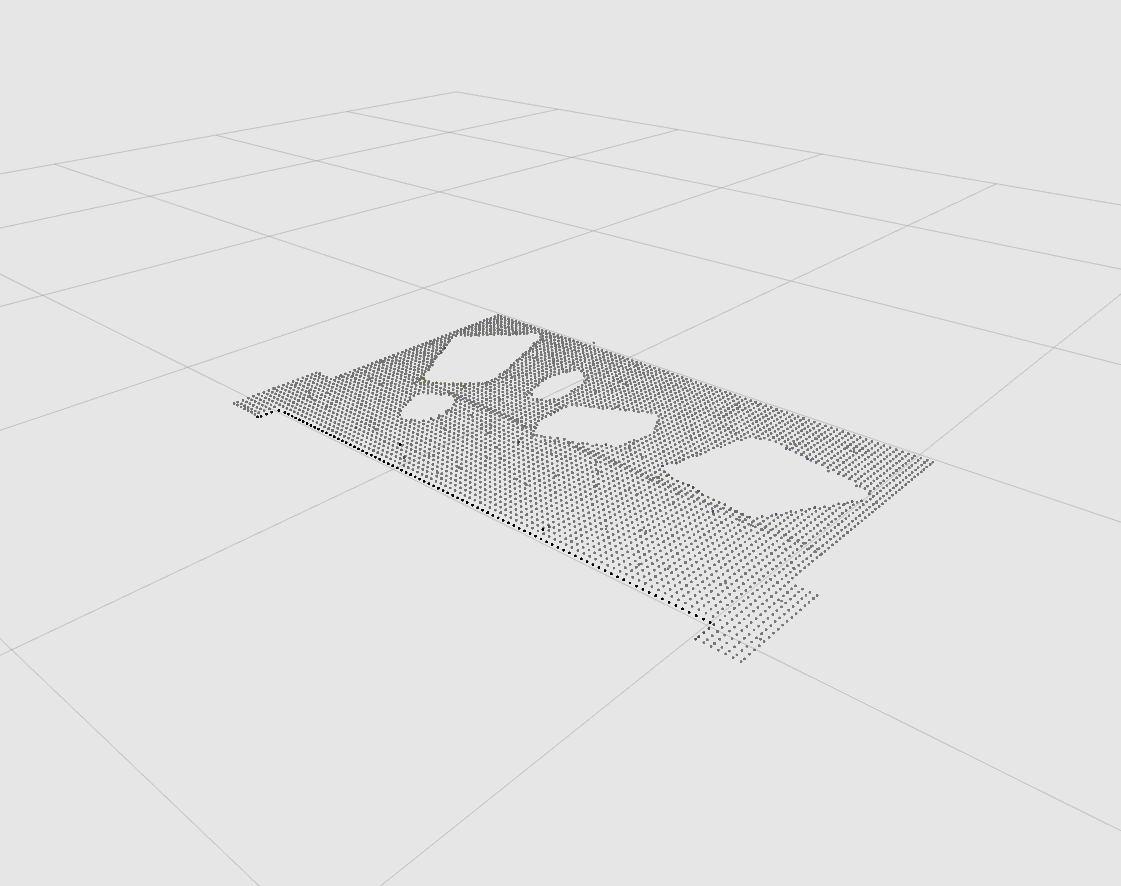
\includegraphics[scale=0.2]{image6}
\caption{Include an image of filtered point cloud table}
\end{minipage}
\hspace{0.5cm}
\begin{minipage}{0.45\linewidth}
\centering
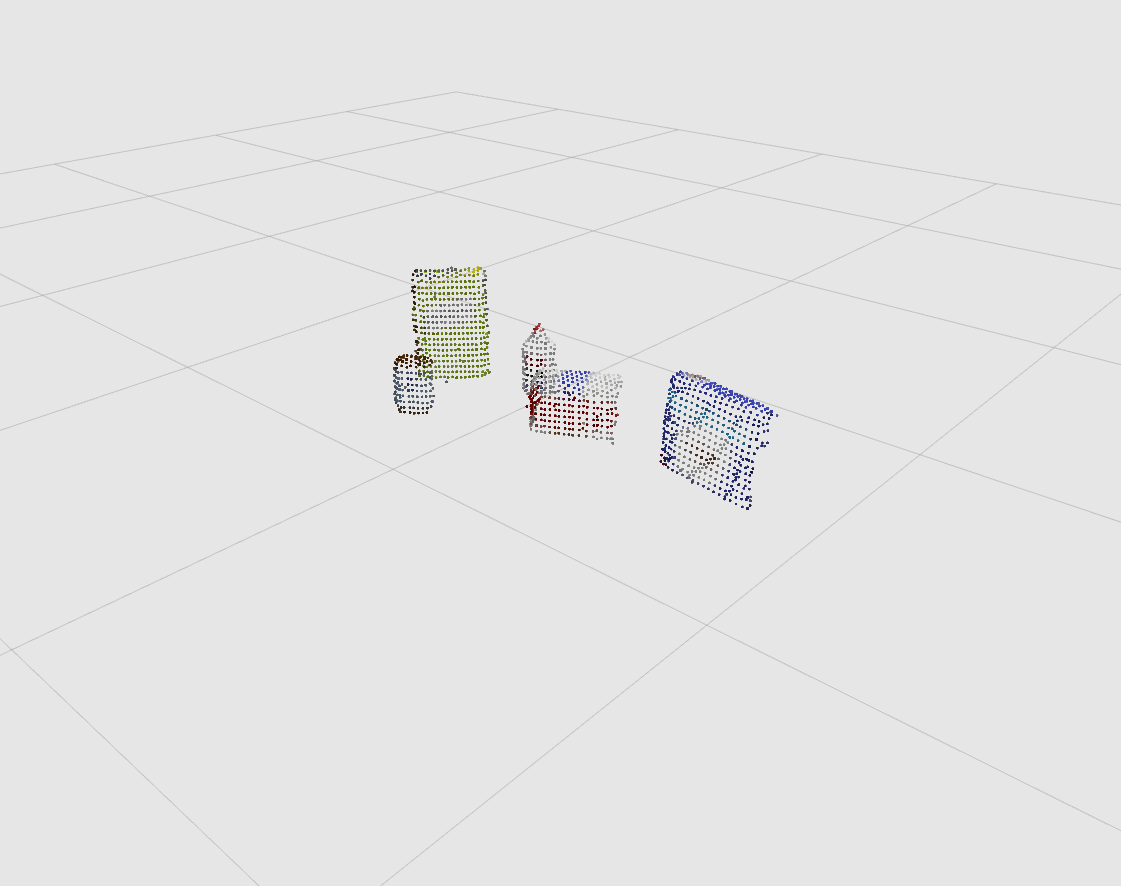
\includegraphics[scale=0.2]{image8}
\caption{Include an image of the filtered point cloud which has all of the objects only}
\end{minipage}
\end{figure}

\newpage

\subsubsection{Euclidean Clustering (DBSCAN)}
Segmentation is undertaken using a Euclidean clustering algorithm called DBSCAN - the implementation can be seen in Listing 5. The algorithm is a density based spatial clustering algorithm. Typically this algorithm is employed when k-means clustering is not appropriate, that is,  points in the point cloud together based on their proximity to each other.

Potential problems with this method. This method encounters problems if the objects are too close to each other. If the objects are too close to each other, then the Euclidean clustering method fails - the algorithm will think that the objects 

\vspace{1cm}

\begin{figure}[h]\scriptsize
\begin{sexylisting}{Apply Euclidean clustering to the pointcloud}
##############################################################################
    # Extract inliers and outliers
##############################################################################
    # Extract inliers
    cloud_table = cloud_filtered.extract(inliers, negative=False)

    # Extract outliers
    cloud_objects = cloud_filtered.extract(inliers, negative=True)


##############################################################################
    # Euclidean Clustering
##############################################################################
    white_cloud = XYZRGB_to_XYZ(cloud_objects)
    tree = white_cloud.make_kdtree()

    # Create a cluster extraction object
    ec = white_cloud.make_EuclideanClusterExtraction()

    # Set tolerances for distance threshold
    # as well as minimum and maximum cluster size (in points)
    ec.set_ClusterTolerance(0.05)
    ec.set_MinClusterSize(50)
    ec.set_MaxClusterSize(3000)

    # Search the k-d tree for clusters
    ec.set_SearchMethod(tree)

    # Extract indices for each of the discovered clusters
    cluster_indices = ec.Extract()
\end{sexylisting}
\end{figure}

\vspace{1cm}

\begin{figure}[h]
\centering
\begin{minipage}{0.45\linewidth}
\centering
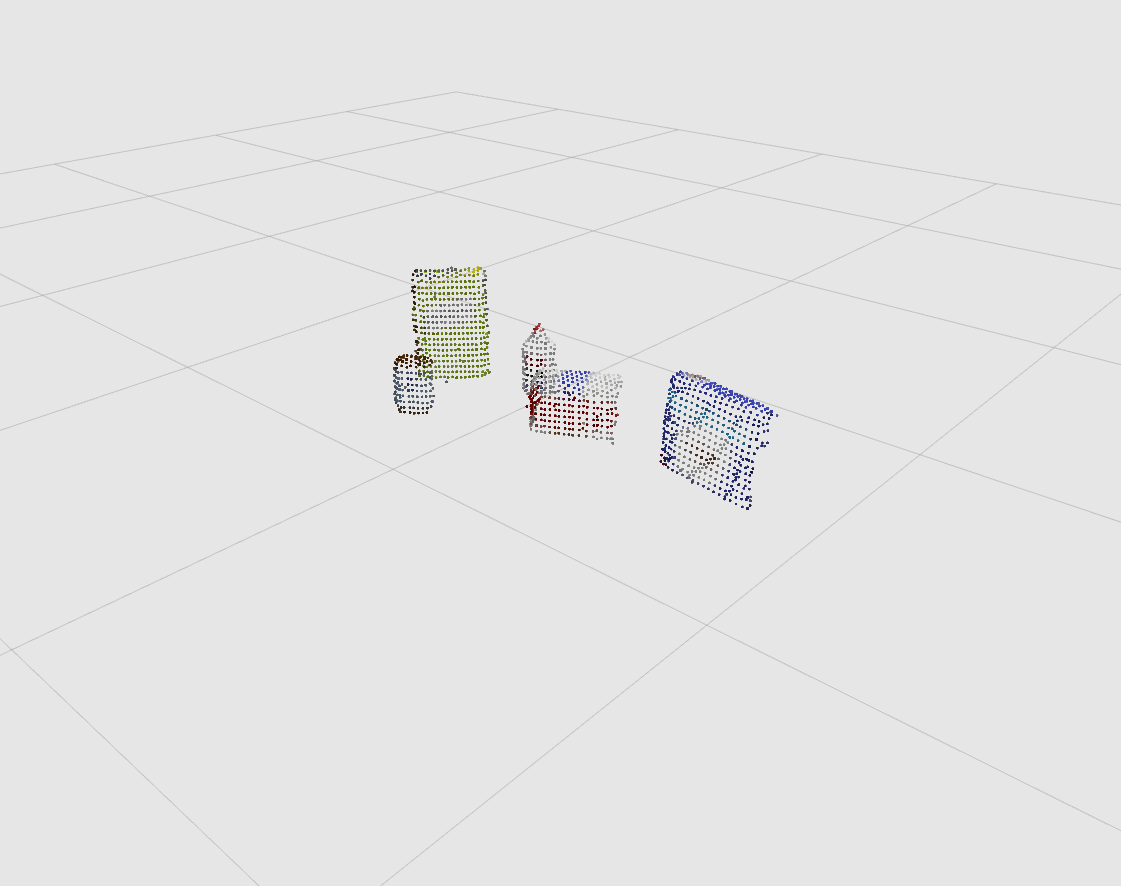
\includegraphics[scale=0.2]{image8}
\caption{Include and image of the unfiltered point cloud}
\end{minipage}
\hspace{0.5cm}
\begin{minipage}{0.45\linewidth}
\centering
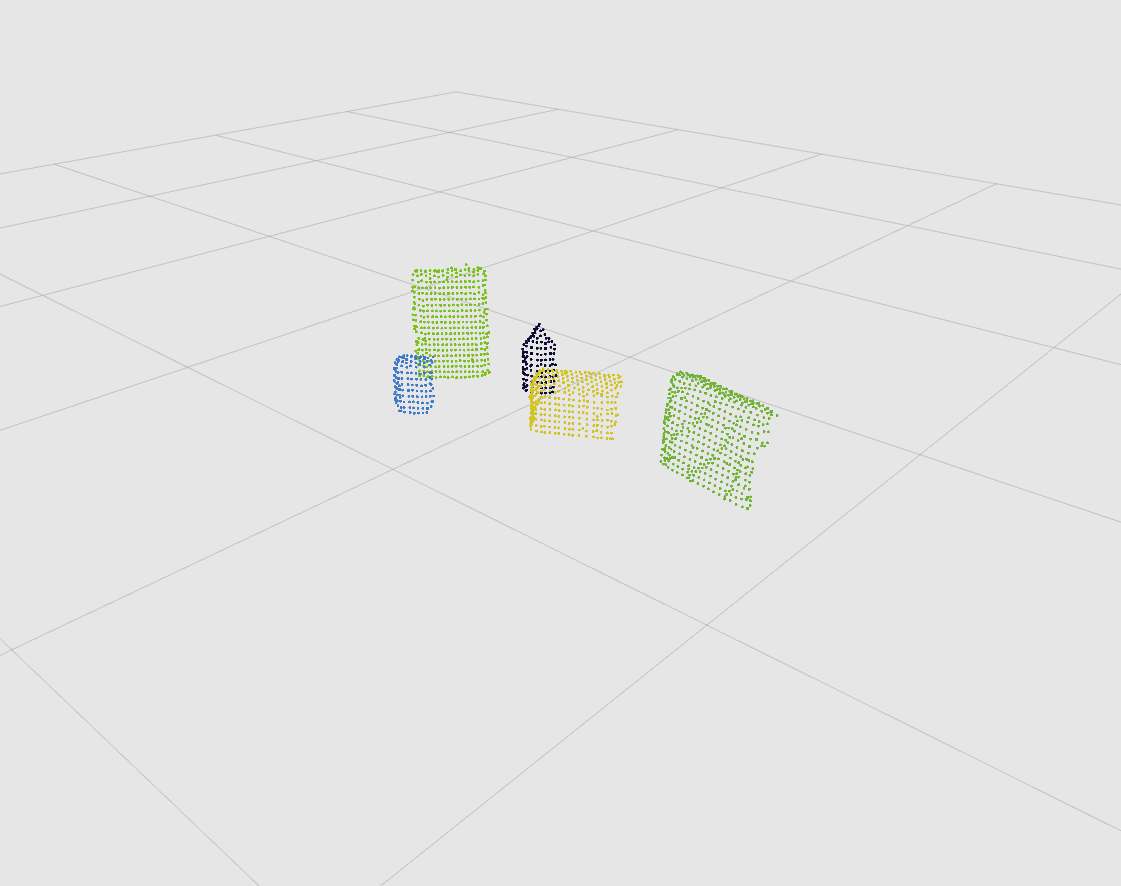
\includegraphics[scale=0.2]{image9}
\caption{Include an image of the filtered point cloud}
\end{minipage}
\end{figure}

\begin{figure}[h]\scriptsize
\begin{sexylisting}{Assign a mask colour to each segment of the segmented point cloud}
##############################################################################
    # Create Cluster-Mask Point Cloud to visualize each cluster separately
##############################################################################
    #Assign a color corresponding to each segmented object in scene
    cluster_color = get_color_list(len(cluster_indices))

    color_cluster_point_list = []

    for j, indices in enumerate(cluster_indices):
        for i, indice in enumerate(indices):
            color_cluster_point_list.append([white_cloud[indice][0],
                                            white_cloud[indice][1],
                                            white_cloud[indice][2],
                                            rgb_to_float(cluster_color[j])])

    #Create new cloud containing all clusters, each with unique color
    cluster_cloud = pcl.PointCloud_PointXYZRGB()
    cluster_cloud.from_list(color_cluster_point_list)
\end{sexylisting}
\end{figure}

\subsection{Object Recognition}
Object recognition allows a robot to correctly locate an object of interest in the environment. The first step to achieving this is for the robot to distinguish between point cloud data which belong to objects, as opposed to pcl data belonging to the environment. This has largely been achieved using Passthrough filtering, and RANSAC plane segmentation. The next step is to identify the set of pcl data points actually belonging to an individual object - this has been achieved using Euclidean Clustering (DBSCAN). With these two things achieved, the task of identifying an object, can be simplified to identifying a set of features in the object point cloud data, which  match the object of interest.\\

This task requires the robot to be able to distinguish between \textbf{XXXX} different objects that may be present in a scene. A typical set of objects placed in a scene is shown in Figure XXXX.
\begin{figure}
\centering
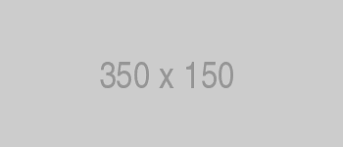
\includegraphics[scale=0.5]{placeholder}
\caption{text}
\end{figure}
%----------------------------------------------
\section{Results \& Conclusion}

%----------------------------------------------
\section{Further Enhancements}


\end{document}